\begin{figure}[ht!]
    \begin{center}
        % This file was created by matlab2tikz.
%
%The latest updates can be retrieved from
%  http://www.mathworks.com/matlabcentral/fileexchange/22022-matlab2tikz-matlab2tikz
%where you can also make suggestions and rate matlab2tikz.
%
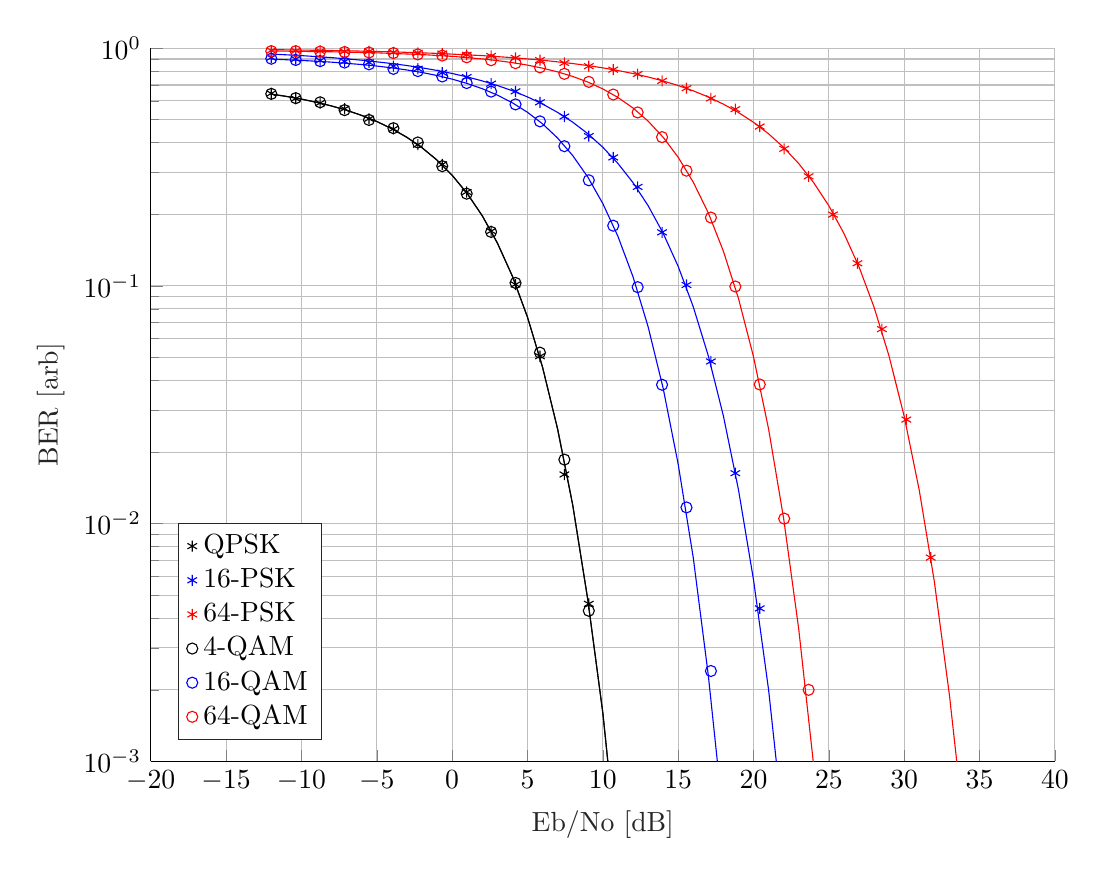
\begin{tikzpicture}

\begin{axis}[%
width=4.521in,
height=3.566in,
at={(0.758in,0.481in)},
scale only axis,
xmin=-20,
xmax=40,
xlabel style={font=\color{white!15!black}},
xlabel={Eb/No [dB]},
ymode=log,
ymin=0.001,
ymax=1,
yminorticks=true,
ylabel style={font=\color{white!15!black}},
ylabel={BER [arb]},
axis background/.style={fill=white},
axis x line*=bottom,
axis y line*=left,
xmajorgrids,
ymajorgrids,
yminorgrids,
legend style={at={(0.03,0.03)}, anchor=south west, legend cell align=left, align=left, draw=white!15!black}
]
\addplot [color=black, only marks, mark=asterisk, mark options={solid, black}]
  table[row sep=crcr]{%
-12	0.644935506449356\\
-10.3793103448276	0.613838616138387\\
-8.75862068965517	0.588141185881412\\
-7.13793103448276	0.556244375562444\\
-5.51724137931035	0.504449555044495\\
-3.89655172413793	0.457454254574543\\
-2.27586206896552	0.392660733926606\\
-0.655172413793103	0.324367563243675\\
0.96551724137931	0.248275172482751\\
2.58620689655172	0.16998300169983\\
4.20689655172414	0.101389861013899\\
5.82758620689655	0.0505949405059495\\
7.44827586206896	0.0160983901609839\\
9.06896551724138	0.0045995400459954\\
};
\addlegendentry{QPSK}

\addplot [color=blue, only marks, mark=asterisk, mark options={solid, blue}]
  table[row sep=crcr]{%
-12	0.911808819118087\\
-10.3793103448276	0.900009999000097\\
-8.75862068965517	0.888211178882111\\
-7.13793103448276	0.879412058794121\\
-5.51724137931035	0.870812918708129\\
-3.89655172413793	0.840015998400157\\
-2.27586206896552	0.819318068193183\\
-0.655172413793103	0.788421157884211\\
0.96551724137931	0.755924407559242\\
2.58620689655173	0.709129087091288\\
4.20689655172414	0.658534146585342\\
5.82758620689655	0.591940805919406\\
7.44827586206896	0.515848415158483\\
9.06896551724138	0.426657334266572\\
10.6896551724138	0.347065293470654\\
12.3103448275862	0.260873912608739\\
13.9310344827586	0.167983201679832\\
15.551724137931	0.100889911008899\\
17.1724137931034	0.0480951904809517\\
18.7931034482759	0.0162983701629837\\
20.4137931034483	0.00439956004399559\\
};
\addlegendentry{16-PSK}

\addplot [color=red, only marks, mark=asterisk, mark options={solid, red}]
  table[row sep=crcr]{%
-12	0.977102289771019\\
-10.3793103448276	0.974602539746022\\
-8.75862068965517	0.972802719728026\\
-7.13793103448276	0.969303069693029\\
-5.51724137931035	0.969003099690034\\
-3.89655172413793	0.960503949605037\\
-2.27586206896552	0.955904409559047\\
-0.655172413793103	0.949005099490047\\
0.96551724137931	0.937706229377065\\
2.58620689655173	0.927407259274075\\
4.20689655172414	0.910408959104092\\
5.82758620689655	0.891110888911112\\
7.44827586206896	0.866313368663131\\
9.06896551724138	0.839916008399158\\
10.6896551724138	0.812018798120188\\
12.3103448275862	0.778222177782225\\
13.9310344827586	0.728127187281273\\
15.551724137931	0.678732126787322\\
17.1724137931034	0.614638536146386\\
18.7931034482759	0.553744625537448\\
20.4137931034483	0.468153184681531\\
22.0344827586207	0.377262273772622\\
23.6551724137931	0.28897110288971\\
25.2758620689655	0.1995800419958\\
26.8965517241379	0.124487551244876\\
28.5172413793103	0.065793420657934\\
30.1379310344828	0.0273972602739727\\
31.7586206896552	0.00719928007199278\\
};
\addlegendentry{64-PSK}

\addplot [color=black, only marks, mark=o, mark options={solid, black}]
  table[row sep=crcr]{%
-12	0.642435756424357\\
-10.3793103448276	0.616238376162385\\
-8.75862068965517	0.592040795920407\\
-7.13793103448276	0.548745125487452\\
-5.51724137931035	0.498950104989501\\
-3.89655172413793	0.460753924607538\\
-2.27586206896552	0.401059894010598\\
-0.655172413793103	0.318968103189681\\
0.96551724137931	0.244275572442756\\
2.58620689655172	0.168683131686831\\
4.20689655172414	0.102889711028897\\
5.82758620689655	0.0523947605239475\\
7.44827586206896	0.0185981401859814\\
9.06896551724138	0.00429957004299569\\
};
\addlegendentry{4-QAM}

\addplot [color=blue, only marks, mark=o, mark options={solid, blue}]
  table[row sep=crcr]{%
-12	0.902809719028099\\
-10.3793103448276	0.892110788921108\\
-8.75862068965517	0.881811818818115\\
-7.13793103448276	0.86991300869913\\
-5.51724137931035	0.855014498550145\\
-3.89655172413793	0.818318168183184\\
-2.27586206896552	0.800719928007198\\
-0.655172413793103	0.760323967603242\\
0.96551724137931	0.713228677132287\\
2.58620689655173	0.656534346565342\\
4.20689655172414	0.580141985801419\\
5.82758620689655	0.492150784921508\\
7.44827586206896	0.387061293870612\\
9.06896551724138	0.278172182781722\\
10.6896551724138	0.17918208179182\\
12.3103448275862	0.0987901209879009\\
13.9310344827586	0.0383961603839615\\
15.551724137931	0.0116988301169883\\
17.1724137931034	0.00239976002399759\\
};
\addlegendentry{16-QAM}

\addplot [color=red, only marks, mark=o, mark options={solid, red}]
  table[row sep=crcr]{%
-12	0.971702829717026\\
-10.3793103448276	0.971502849715032\\
-8.75862068965517	0.967503249675034\\
-7.13793103448276	0.963203679632034\\
-5.51724137931035	0.958904109589043\\
-3.89655172413793	0.953704629537047\\
-2.27586206896552	0.94150584941506\\
-0.655172413793103	0.930506949305068\\
0.96551724137931	0.915408459154082\\
2.58620689655173	0.889811018898108\\
4.20689655172414	0.864813518648134\\
5.82758620689655	0.830316968303166\\
7.44827586206896	0.779922007799218\\
9.06896551724138	0.72152784721528\\
10.6896551724138	0.63823617638236\\
12.3103448275862	0.536646335366465\\
13.9310344827586	0.422557744225577\\
15.551724137931	0.305269473052695\\
17.1724137931034	0.193880611938807\\
18.7931034482759	0.0993900609939009\\
20.4137931034483	0.0384961503849614\\
22.0344827586207	0.0104989501049895\\
23.6551724137931	0.00199980001999799\\
};
\addlegendentry{64-QAM}

\addplot [color=black, forget plot]
  table[row sep=crcr]{%
-12	0.641\\
-11	0.6267\\
-10	0.610500000000001\\
-9	0.592099999999999\\
-8	0.571300000000001\\
-7	0.547800000000001\\
-6	0.5213\\
-5	0.4915\\
-4	0.458399999999999\\
-3	0.421600000000001\\
-2	0.381399999999999\\
-1	0.3381\\
0	0.2921\\
1	0.2447\\
2	0.1972\\
3	0.1516\\
4	0.1098\\
5	0.0739\\
6	0.0455\\
7	0.025\\
8	0.012\\
9	0.0048\\
10	0.0016\\
10.8192189328474	0.000501187233627271\\
};
\addplot [color=black, forget plot]
  table[row sep=crcr]{%
-12	0.641\\
-11	0.6267\\
-10	0.610500000000001\\
-9	0.592099999999999\\
-8	0.571300000000001\\
-7	0.547800000000001\\
-6	0.5213\\
-5	0.4915\\
-4	0.458399999999999\\
-3	0.421600000000001\\
-2	0.381399999999999\\
-1	0.3381\\
0	0.2921\\
1	0.2447\\
2	0.1972\\
3	0.1516\\
4	0.1098\\
5	0.0739\\
6	0.0455\\
7	0.025\\
8	0.012\\
9	0.0048\\
10	0.0016\\
10.8192189328474	0.000501187233627271\\
};
\addplot [color=blue, forget plot]
  table[row sep=crcr]{%
-12	0.944700000000002\\
-10	0.930500000000003\\
-8	0.912499999999998\\
-6	0.889999999999997\\
-4	0.861800000000001\\
-3	0.845100000000001\\
-2	0.826500000000003\\
-1	0.805799999999998\\
0	0.782599999999998\\
1	0.756899999999999\\
2	0.728300000000001\\
3	0.6967\\
4	0.6619\\
5	0.623700000000002\\
6	0.582000000000001\\
7	0.536800000000001\\
8	0.488300000000001\\
9	0.436800000000001\\
10	0.382999999999999\\
11	0.327600000000001\\
12	0.271999999999999\\
13	0.217800000000001\\
14	0.1667\\
15	0.1208\\
16	0.0816999999999997\\
17	0.0507999999999999\\
18	0.0284\\
19	0.0138999999999999\\
20	0.00580000000000002\\
21	0.002\\
22	0.000513970000000001\\
};
\addplot [color=blue, forget plot]
  table[row sep=crcr]{%
-12	0.899500000000003\\
-10	0.8882\\
-8	0.873300000000002\\
-6	0.853299999999999\\
-5	0.840899999999999\\
-4	0.826400000000001\\
-3	0.809600000000001\\
-2	0.7901\\
-1	0.767299999999998\\
0	0.741\\
1	0.710400000000001\\
2	0.675199999999998\\
3	0.634800000000001\\
4	0.5889\\
5	0.537400000000001\\
6	0.480399999999998\\
7	0.4187\\
8	0.353499999999999\\
9	0.287099999999999\\
10	0.222\\
11	0.1617\\
12	0.1094\\
13	0.0675000000000001\\
14	0.0371999999999999\\
15	0.0177999999999999\\
16	0.00720000000000001\\
17	0.0023\\
18	0.000572640000000001\\
};
\addplot [color=red, forget plot]
  table[row sep=crcr]{%
-12	0.986100000000007\\
-7	0.975299999999993\\
-4	0.965100000000003\\
-1	0.950700000000004\\
2	0.930400000000004\\
4	0.912400000000003\\
6	0.889900000000001\\
8	0.861599999999995\\
9	0.844899999999996\\
10	0.826300000000003\\
11	0.805499999999999\\
12	0.782400000000001\\
13	0.756600000000001\\
14	0.727999999999995\\
15	0.696400000000004\\
16	0.661500000000001\\
17	0.623199999999998\\
18	0.581500000000002\\
19	0.536299999999998\\
20	0.4877\\
21	0.436199999999999\\
22	0.3823\\
23	0.326999999999999\\
24	0.271399999999998\\
25	0.217199999999999\\
26	0.1662\\
27	0.120299999999999\\
28	0.0812999999999996\\
29	0.0505000000000003\\
30	0.0282\\
31	0.0138\\
32	0.00569999999999995\\
33	0.00189999999999998\\
34	0.000505460000000002\\
};
\addplot [color=red, forget plot]
  table[row sep=crcr]{%
-12	0.973300000000002\\
-8	0.965600000000003\\
-5	0.9557\\
-2	0.939799999999997\\
0	0.923699999999997\\
2	0.901100000000004\\
3	0.8865\\
4	0.869200000000002\\
5	0.848499999999997\\
6	0.823899999999998\\
7	0.794799999999997\\
8	0.760500000000001\\
9	0.720399999999998\\
10	0.673799999999998\\
11	0.620500000000001\\
12	0.560299999999998\\
13	0.493699999999999\\
14	0.422100000000001\\
15	0.347600000000001\\
16	0.273200000000001\\
17	0.2027\\
18	0.14\\
19	0.0886000000000002\\
20	0.0503\\
21	0.025\\
22	0.0105\\
23	0.0036\\
24	0.00095029\\
};
\end{axis}
\end{tikzpicture}%
        \caption{Comparison of BER for QPSK, 16PSK, 64PSK, 16QAM and 64QAM}
    \end{center}\label{fig:3}
\end{figure}

\tiny

\begin{equation} \label{eq:Q_function}
    Q\left(x\right)\ =\ \frac{1}{2}\cdot\operatorname{erf}c\left(\frac{x}{\sqrt{2\cdot\log_{2}\left(M\right)}}\right)
\end{equation}

\begin{equation}\label{eq:PSK_QAM}
    \begin{split}
        BER_{QPSK}&=2Q\left(\sqrt{2\cdot\frac{E_{b}}{N_{0}}}\right)-Q^{2}\left(\sqrt{2\cdot\frac{E_{b}}{N_{0}}}\right)\\
        BER_{MPSK}\left(M>4\right)&=2Q\left(\sin\left(\frac{\pi}{M}\right)\cdot\sqrt{2\cdot\frac{E_{b}}{N_{0}}}\right)\\
        BER_{MQAM}&=1-\left(1-2\left(1-\frac{1}{\sqrt{M}}\right)\cdot Q\left(\sqrt{\frac{3\cdot\log_{2}\left(M\right)\cdot\frac{E_{b}}{N_{0}}}{M-1}}\right)\right)^{2}
    \end{split}
\end{equation}

\normalsize

An adaption of \cite{Mathuranathan2020Nov} was used to define the equations for BER as shown in eq.~\eqref{eq:PSK_QAM} where the Q function is defined in eq.~\eqref{eq:Q_function}. 

Figure~\ref{fig:3} shows the theoretical (continuous) vs simulated (discrete) BER for QPSK, 16PSK, 64PSK, 16QAM and 64QAM. The results are obtained using the Matlab script as shown in \ref{matlabs:task3}, where the stop time was set to 2000 for the simulated results. The Graph shows the simulated results have very little variation from the theoretical results.

The equation for QAM BER is only correct for square numbers of M. A bit error usually error occurs when a symbol is mistaken for its nearest member. The distance between symbols on the constellation diagram is variable for 8-QAM. Therefore the error for each BER for each symbol would have to be calculated and averaged, which is much more complicated than for a square number of M with a constant inter-symbol distance.